\documentclass[10pt]{article}
\usepackage[ansinew]{inputenc}
\usepackage{latexsym,bezier,enumerate,longtable,dcolumn,color,pstricks,xspace,curves,mathpazo,url,xcolor}
\usepackage{amsmath,amsthm,amsopn,amstext,amscd,amsfonts,amssymb,fancybox,pst-node,pst-tree}
\usepackage{tikz}
\usetikzlibrary{positioning}

\begin{document}

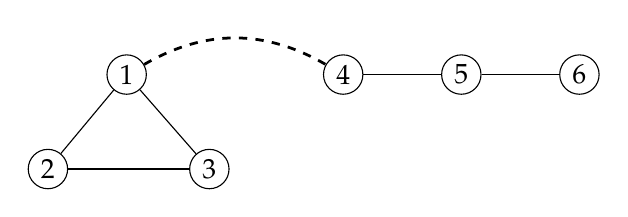
\begin{tikzpicture}[node_style/.style={draw,circle,minimum size=0.5cm,inner sep=1}]
\node[node_style] (uno) at (9,1.2) {1} ;
\node[node_style] (dos) at (8.0,0.0) {2} ;
\node[node_style] (tres) at (10.05,0.0) {3} ;
\node[node_style] (cuatro) at (11.75,1.2) {4} ;
\node[node_style] (cinco) at (13.25,1.2) {5} ;
\node[node_style] (seis) at (14.75,1.2) {6} ;
\draw (uno) -- (dos);
\draw (dos) -- (tres);
\draw (tres) -- (uno);
\draw (cuatro) -- (cinco);
\draw (cinco) -- (seis);
\draw [dashed,line width=1.0pt] (uno) edge[-,bend left=30]  (cuatro);
\end{tikzpicture}

\end{document}